%Version 3.1 December 2024
% See section 11 of the User Manual for version history
%
%%%%%%%%%%%%%%%%%%%%%%%%%%%%%%%%%%%%%%%%%%%%%%%%%%%%%%%%%%%%%%%%%%%%%%
%%                                                                 %%
%% Please do not use \input{...} to include other tex files.       %%
%% Submit your LaTeX manuscript as one .tex document.              %%
%%                                                                 %%
%% All additional figures and files should be attached             %%
%% separately and not embedded in the \TeX\ document itself.       %%
%%                                                                 %%
%%%%%%%%%%%%%%%%%%%%%%%%%%%%%%%%%%%%%%%%%%%%%%%%%%%%%%%%%%%%%%%%%%%%%

%%\documentclass[referee,sn-basic]{sn-jnl}% referee option is meant for double line spacing

%%=======================================================%%
%% to print line numbers in the margin use lineno option %%
%%=======================================================%%

%%\documentclass[lineno,pdflatex,sn-basic]{sn-jnl}% Basic Springer Nature Reference Style/Chemistry Reference Style

%%=========================================================================================%%
%% the documentclass is set to pdflatex as default. You can delete it if not appropriate.  %%
%%=========================================================================================%%

%%\documentclass[sn-basic]{sn-jnl}% Basic Springer Nature Reference Style/Chemistry Reference Style

%%Note: the following reference styles support Namedate and Numbered referencing. By default the style follows the most common style. To switch between the options you can add or remove “Numbered” in the optional parenthesis. 
%%The option is available for: sn-basic.bst, sn-chicago.bst%  
 
%%\documentclass[pdflatex,sn-nature]{sn-jnl}% Style for submissions to Nature Portfolio journals
%%\documentclass[pdflatex,sn-basic]{sn-jnl}% Basic Springer Nature Reference Style/Chemistry Reference Style
\documentclass[pdflatex,sn-mathphys-num]{sn-jnl}% Math and Physical Sciences Numbered Reference Style
%%\documentclass[pdflatex,sn-mathphys-ay]{sn-jnl}% Math and Physical Sciences Author Year Reference Style
%%\documentclass[pdflatex,sn-aps]{sn-jnl}% American Physical Society (APS) Reference Style
%%\documentclass[pdflatex,sn-vancouver-num]{sn-jnl}% Vancouver Numbered Reference Style
%%\documentclass[pdflatex,sn-vancouver-ay]{sn-jnl}% Vancouver Author Year Reference Style
%%\documentclass[pdflatex,sn-apa]{sn-jnl}% APA Reference Style
%%\documentclass[pdflatex,sn-chicago]{sn-jnl}% Chicago-based Humanities Reference Style

%%%% Standard Packages
%%<additional latex packages if required can be included here>

\usepackage{graphicx}%
\usepackage{multirow}%
\usepackage{amsmath,amssymb,amsfonts}%
\usepackage{amsthm}%
\usepackage{mathrsfs}%
\usepackage[title]{appendix}%
\usepackage{xcolor}%
\usepackage{textcomp}%
\usepackage{manyfoot}%
\usepackage{booktabs}%
\usepackage{algorithm}%
\usepackage{algorithmicx}%
\usepackage{algpseudocode}%
\usepackage{listings}%
%%%%

%%%%%=============================================================================%%%%
%%%%  Remarks: This template is provided to aid authors with the preparation
%%%%  of original research articles intended for submission to journals published 
%%%%  by Springer Nature. The guidance has been prepared in partnership with 
%%%%  production teams to conform to Springer Nature technical requirements. 
%%%%  Editorial and presentation requirements differ among journal portfolios and 
%%%%  research disciplines. You may find sections in this template are irrelevant 
%%%%  to your work and are empowered to omit any such section if allowed by the 
%%%%  journal you intend to submit to. The submission guidelines and policies 
%%%%  of the journal take precedence. A detailed User Manual is available in the 
%%%%  template package for technical guidance.
%%%%%=============================================================================%%%%

%% as per the requirement new theorem styles can be included as shown below
\theoremstyle{thmstyleone}%
\newtheorem{theorem}{Theorem}%  meant for continuous numbers
%%\newtheorem{theorem}{Theorem}[section]% meant for sectionwise numbers
%% optional argument [theorem] produces theorem numbering sequence instead of independent numbers for Proposition
\newtheorem{proposition}[theorem]{Proposition}% 
%%\newtheorem{proposition}{Proposition}% to get separate numbers for theorem and proposition etc.

\theoremstyle{thmstyletwo}%
\newtheorem{example}{Example}%
\newtheorem{remark}{Remark}%

\theoremstyle{thmstylethree}%
\newtheorem{definition}{Definition}%

\raggedbottom
%%\unnumbered% uncomment this for unnumbered level heads

\begin{document}

\title[Quantum HPC Simulation]{High-Performance Quantum Simulation for Scalable Quantum Machine Learning}

%%=============================================================%%
%% GivenName	-> \fnm{Joergen W.}
%% Particle	-> \spfx{van der} -> surname prefix
%% FamilyName	-> \sur{Ploeg}
%% Suffix	-> \sfx{IV}
%% \author*[1,2]{\fnm{Joergen W.} \spfx{van der} \sur{Ploeg} 
%%  \sfx{IV}}\email{iauthor@gmail.com}
%%=============================================================%%

\author*[1,2]{\fnm{Kyle} \sur{Hartness}}\email{kahartne@utica.edu}

\author[2,3]{\fnm{Sofia} \sur{Furda}}\email{soffurda@gmail.com}

\author[1,2]{\fnm{Edmund} \sur{Bombardieri}}\email{ebombardieri@mail.wlu.edu}

\affil*[1]{\orgdiv{...}, \orgname{Utica University}, \orgaddress{\street{Burrstone Rd}, \city{Utica}, \postcode{13504}, \state{NY}, \country{USA}}}

\affil[2]{\orgdiv{Department}, \orgname{Organization}, \orgaddress{\street{Street}, \city{City}, \postcode{10587}, \state{State}, \country{Country}}}

\affil[3]{\orgdiv{Department}, \orgname{Organization}, \orgaddress{\street{Street}, \city{City}, \postcode{610101}, \state{State}, \country{Country}}}

%%==================================%%
%% Sample for unstructured abstract %%
%%==================================%%

\abstract{
    Quantum computing has the potential to provide new approaches to machine learning and data processing, but practical quantum workloads remain constrained by simulation cost, limited hardware resources, and the difficulty of scaling experiments across heterogeneous computing environments. This project investigates a high-performance computing (HPC) workflow for quantum machine learning simulations using Qiskit Aer and HPC resources. The work combines quantum feature-map construction, controlled simulation experiments, MPI-based parallelization, GPU acceleration experiments, and distributed execution on platforms such as Bridges-2. The project is organized into complementary tracks that address quantum-kernel development, HPC parallelization and benchmarking, and application-level data processing. During the first five weeks, the team established the simulation framework, implemented and validated a gate-by-gate construction of the ZZFeatureMap, established an MPI execution environment on Bridges-2, and completed an initial 12-condition parameter sweep. These results provide a baseline for larger-scale, GPU, cross-resource, and dataset-extension experiments planned for the remaining project period.
    }

%%================================%%
%% Sample for structured abstract %%
%%================================%%

% \abstract{\textbf{Purpose:} The abstract serves both as a general introduction to the topic and as a brief, non-technical summary of the main results and their implications. The abstract must not include subheadings (unless expressly permitted in the journal's Instructions to Authors), equations or citations. As a guide the abstract should not exceed 200 words. Most journals do not set a hard limit however authors are advised to check the author instructions for the journal they are submitting to.
% 
% \textbf{Methods:} The abstract serves both as a general introduction to the topic and as a brief, non-technical summary of the main results and their implications. The abstract must not include subheadings (unless expressly permitted in the journal's Instructions to Authors), equations or citations. As a guide the abstract should not exceed 200 words. Most journals do not set a hard limit however authors are advised to check the author instructions for the journal they are submitting to.
% 
% \textbf{Results:} The abstract serves both as a general introduction to the topic and as a brief, non-technical summary of the main results and their implications. The abstract must not include subheadings (unless expressly permitted in the journal's Instructions to Authors), equations or citations. As a guide the abstract should not exceed 200 words. Most journals do not set a hard limit however authors are advised to check the author instructions for the journal they are submitting to.
% 
% \textbf{Conclusion:} The abstract serves both as a general introduction to the topic and as a brief, non-technical summary of the main results and their implications. The abstract must not include subheadings (unless expressly permitted in the journal's Instructions to Authors), equations or citations. As a guide the abstract should not exceed 200 words. Most journals do not set a hard limit however authors are advised to check the author instructions for the journal they are submitting to.}

\keywords{quantum computing, quantum machine learning, high-performance computing, Qiskit Aer, MPI, GPU acceleration}

%%\pacs[JEL Classification]{D8, H51}

%%\pacs[MSC Classification]{35A01, 65L10, 65L12, 65L20, 65L70}

\maketitle

\section{Introduction}\label{sec1}

Quantum computing has emerged as a potential approach for addressing computational problems that are difficult to solve efficiently using conventional methods. One area of interest is quantum machine learning (QML), where classical data can be encoded into quantum states and processed using parameterized quantum circuits. Quantum feature maps provide one approach for embedding classical feature vectors into quantum states, enabling the construction of quantum kernels and other QML methods \cite{havlicek2019}. However, the computational cost of simulating quantum circuits increases rapidly as the number of qubits and circuit complexity grow, creating a need for efficient simulation and high-performance computing resources.

The research problem addressed by this project is how to develop and evaluate a scalable computational workflow for quantum machine learning simulations across heterogeneous computing environments. In particular, the project investigates how quantum simulation workloads can be organized, parallelized, and benchmarked using conventional CPUs, GPUs, and distributed HPC resources. The goal is not only to execute a quantum circuit successfully, but to establish an experimental framework that can measure performance, scalability, and the effects of different simulation and system configurations.

The project is divided into complementary tracks that contribute different components to this research problem. The quantum-computing track establishes the quantum feature-map and simulation methodology, including the construction and validation of the ZZFeatureMap and its manual gate-by-gate equivalent. The HPC track develops the computational infrastructure required to execute and benchmark these workloads, including MPI experimentation, SLURM-based execution, and testing on Bridges-2. The application and data-processing track provides the datasets and processing workflow needed to connect the quantum simulation to practical machine-learning experiments. Together, these tracks provide the components necessary to evaluate how quantum machine-learning workloads can be executed and scaled in an HPC environment.

During the first five weeks of the project, the team established the initial quantum simulation framework, developed the dataset and preprocessing pipeline, implemented the quantum feature-map construction, and validated a manual circuit implementation. The HPC work progressed from MPI environment setup to a working SLURM parameter-sweep workflow on Bridges-2. By the end of Week 5, a parameter sweep covering four values of $\epsilon$ and three simulation conditions had been completed, providing an initial experimental baseline for the subsequent parallelization and benchmarking work.

\section{Experimental Framework and Current Results}\label{sec2}

\subsection{Quantum Simulation Framework}\label{subsec:framework}

The QuantumHPC framework was developed as a modular workflow connecting dataset processing, quantum feature-map construction, quantum simulation, and experiment logging. The current implementation loads the configured dataset, extracts the numerical feature representation, constructs the quantum feature map, executes the simulation, and records the resulting experimental configuration and runtime information.

The quantum circuit component implements the ZZFeatureMap in two forms. The first uses the Qiskit circuit-library implementation, while the second constructs the feature map manually from primitive quantum gates. The manual implementation was developed to provide a gate-level representation of the circuit and to validate the behavior of the library implementation without relying exclusively on a high-level circuit-construction shortcut. Both representations are used within the same experimental framework.

The simulation layer is based on Qiskit Aer and supports the project's quantum simulation conditions \cite{qiskitaer2025}. The current experiment configuration distinguishes between noiseless simulation, depolarizing noise, and amplitude-damping noise. These simulation conditions represent quantum hardware-noise models and are treated separately from the differential-privacy parameter $\epsilon$. The experiment configuration currently evaluates $\epsilon \in \{1,2,4,8\}$ with $\delta = 10^{-5}$.

\subsection{HPC Execution Environment}\label{subsec:hpc}

The HPC component of the project was developed using the Bridges-2 computing environment. During the initial HPC development phase, an MPI environment was established and tested using a basic C MPI program. Four MPI processes were successfully executed on a Bridges-2 compute node, establishing the project's ability to compile and execute MPI workloads in the target environment. A SLURM-based parameter-sweep workflow was then developed to connect the experiment configuration to the Bridges-2 execution environment.

The parameter-sweep workflow was designed around the four epsilon values $\epsilon = \{1,2,4,8\}$ and three simulation conditions: noiseless, depolarizing, and amplitude-damping. This produced a total of 12 experimental conditions. The Week 5 experiment connected this workflow to the QuantumHPC experiment framework and completed the planned set of Bridges-2 experiments.

\subsection{Bridges-2 Parameter Sweep}\label{subsec:parameter-sweep}

The completed Bridges-2 parameter sweep evaluated four values of the differential-privacy parameter, $\epsilon \in \{1,2,4,8\}$, under three quantum-simulation conditions: noiseless, depolarizing noise, and amplitude-damping noise. This produced twelve experimental configurations executed through the SLURM-based workflow.

Figure~\ref{fig:simulation-time-epsilon} shows the measured CPU simulation time across the four epsilon values. The results demonstrate that simulation time varies substantially across both epsilon values and simulation conditions. The amplitude-damping condition remained comparatively low across the tested values, while the depolarizing and noiseless conditions exhibited larger variations in runtime. In particular, the depolarizing condition reached its highest measured runtime at $\epsilon=2$, whereas the noiseless condition varied from approximately 22~ms at $\epsilon=2$ to approximately 101~ms at $\epsilon=1$.

\begin{figure}[htbp]
    \centering
    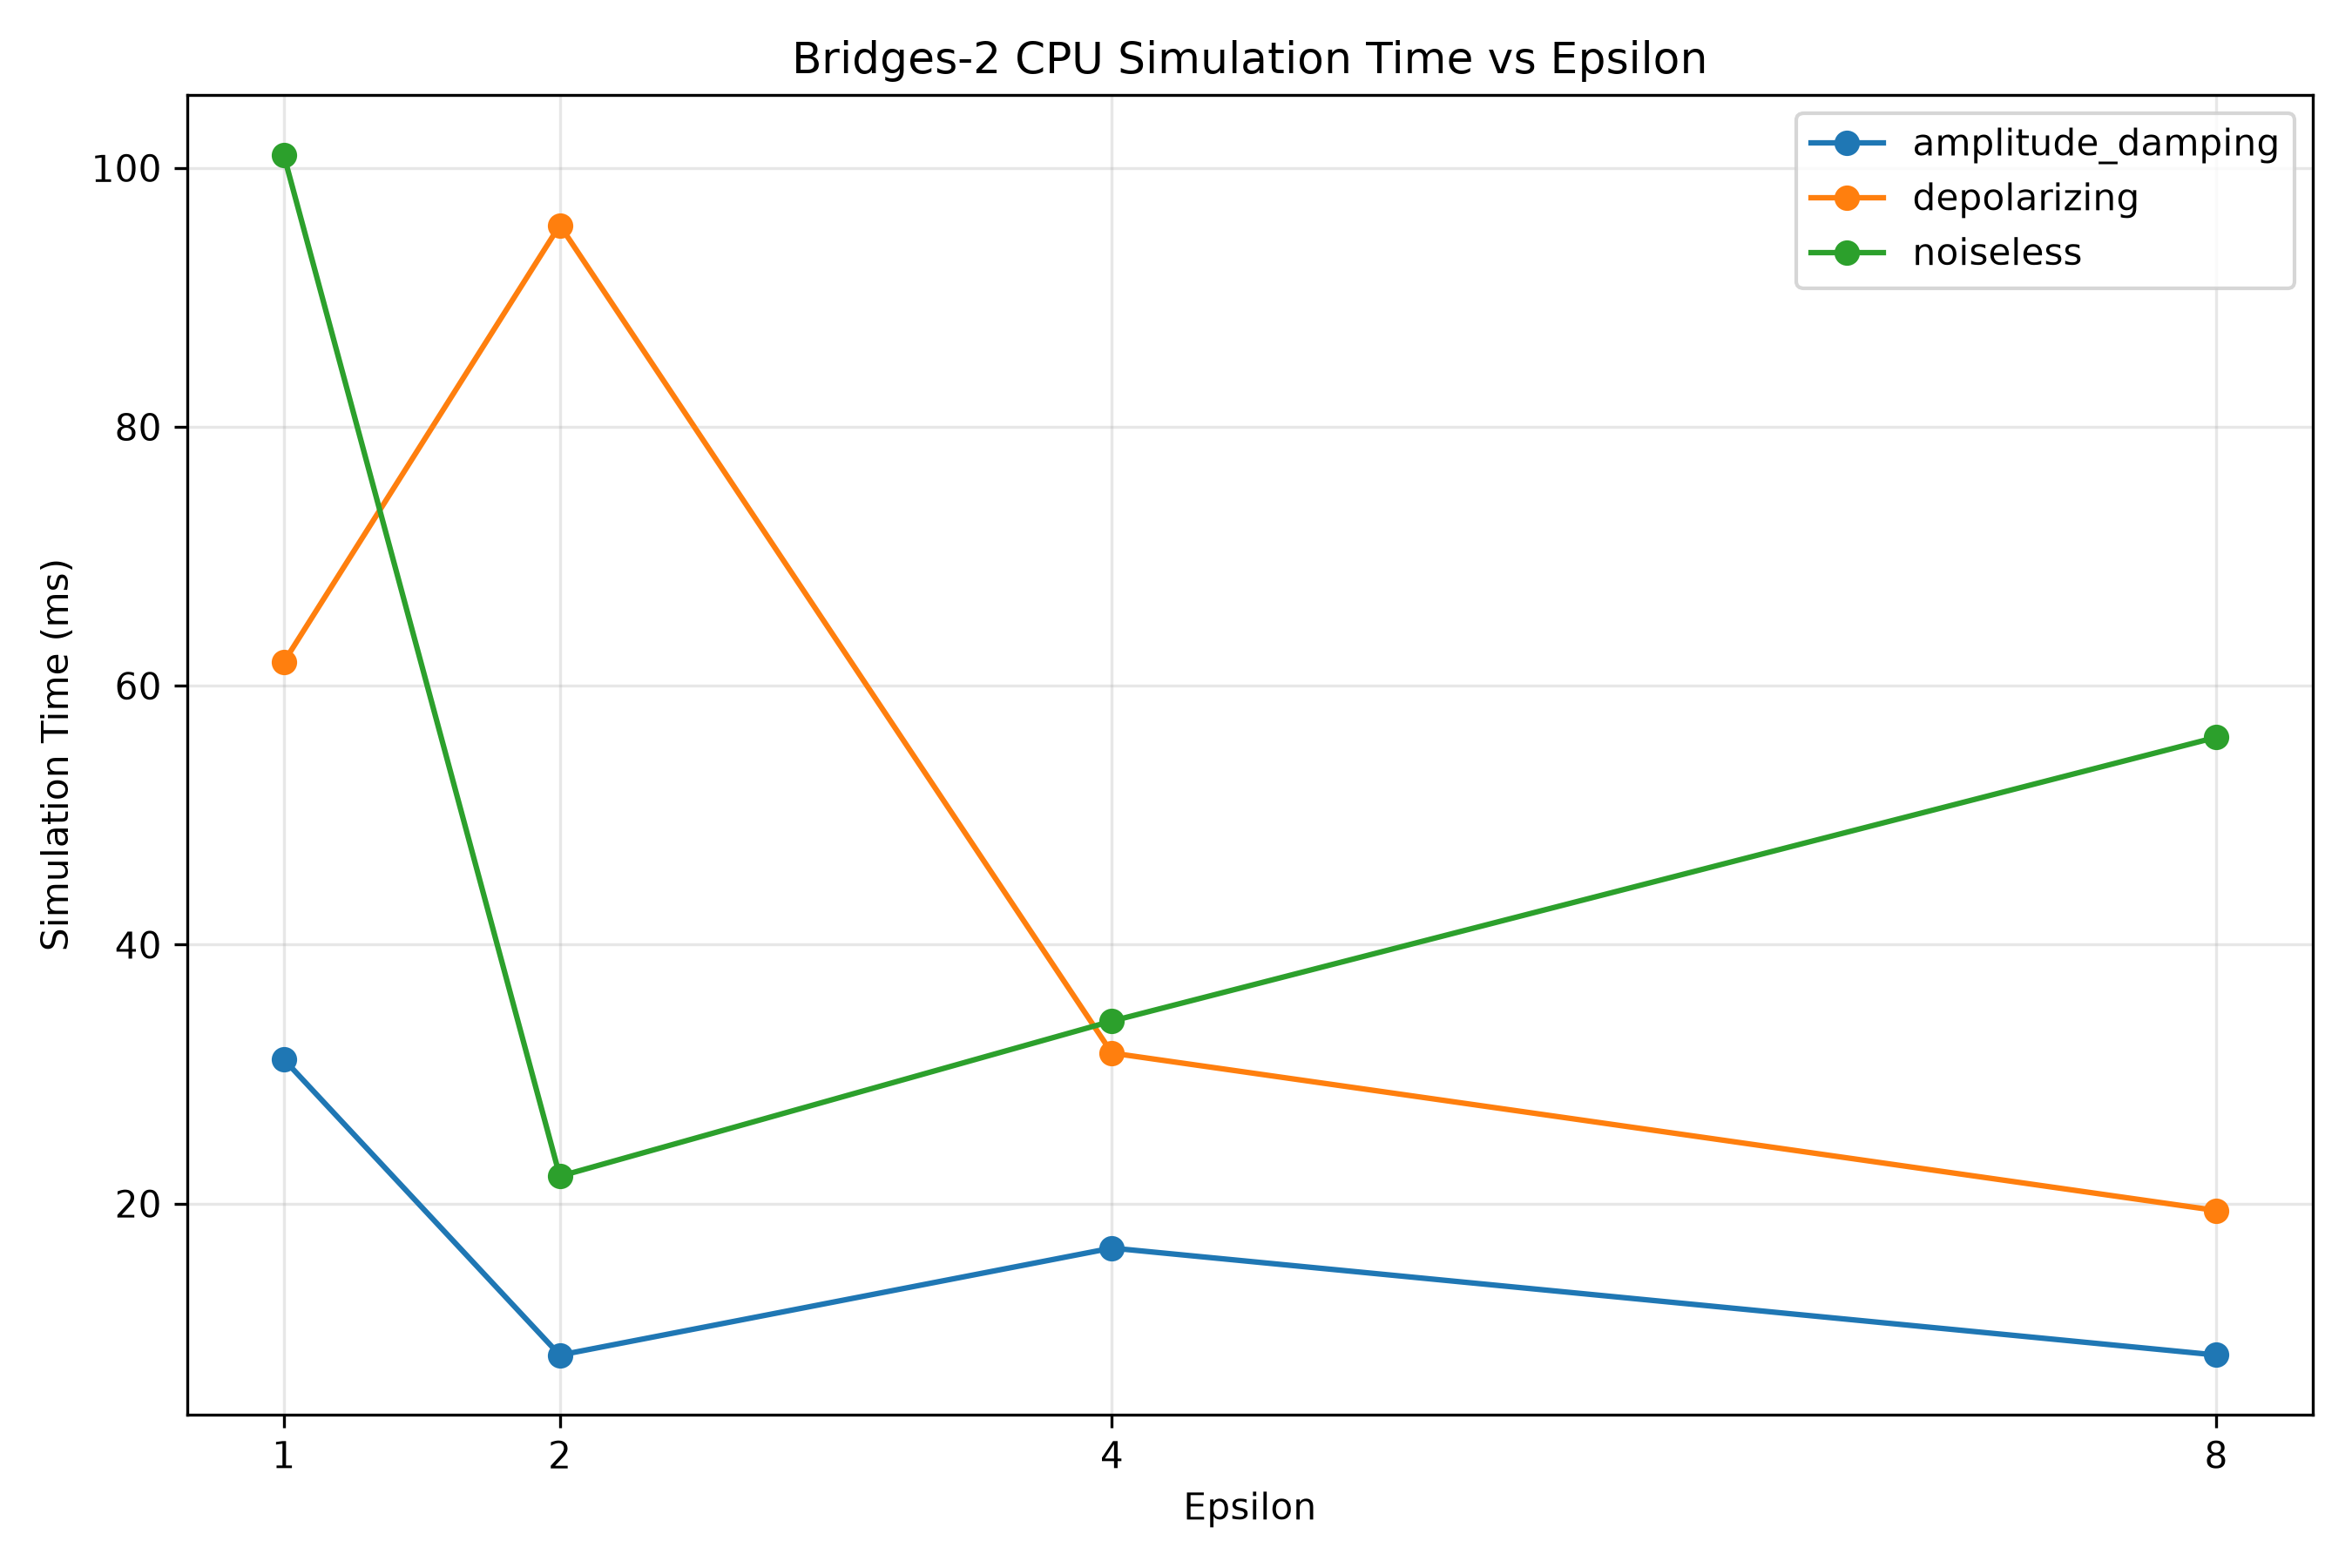
\includegraphics[width=\textwidth]{figures/simulation_time_vs_epsilon.png}
    \caption{Bridges-2 CPU simulation time as a function of $\epsilon$ for noiseless, depolarizing-noise, and amplitude-damping conditions.}
    \label{fig:simulation-time-epsilon}
\end{figure}

These measurements establish an empirical CPU baseline for the simulation workload. Because the runtime does not exhibit a simple monotonic relationship with $\epsilon$, the results also demonstrate the importance of measuring each experimental configuration rather than assuming that increasing or decreasing $\epsilon$ will directly determine simulation cost.

\subsection{MPI Scaling on Bridges-2}\label{subsec:mpi-scaling}

To evaluate the effect of distributed execution, the quantum-simulation workload was tested using 1, 2, and 4 MPI processes on Bridges-2. Figure~\ref{fig:mpi-runtime} shows the measured mean wall time as the number of MPI processes increased. The mean runtime decreased from approximately 6.1~s with one process to approximately 3.5~s with two processes and approximately 2.3~s with four processes.

\begin{figure}[htbp]
    \centering
    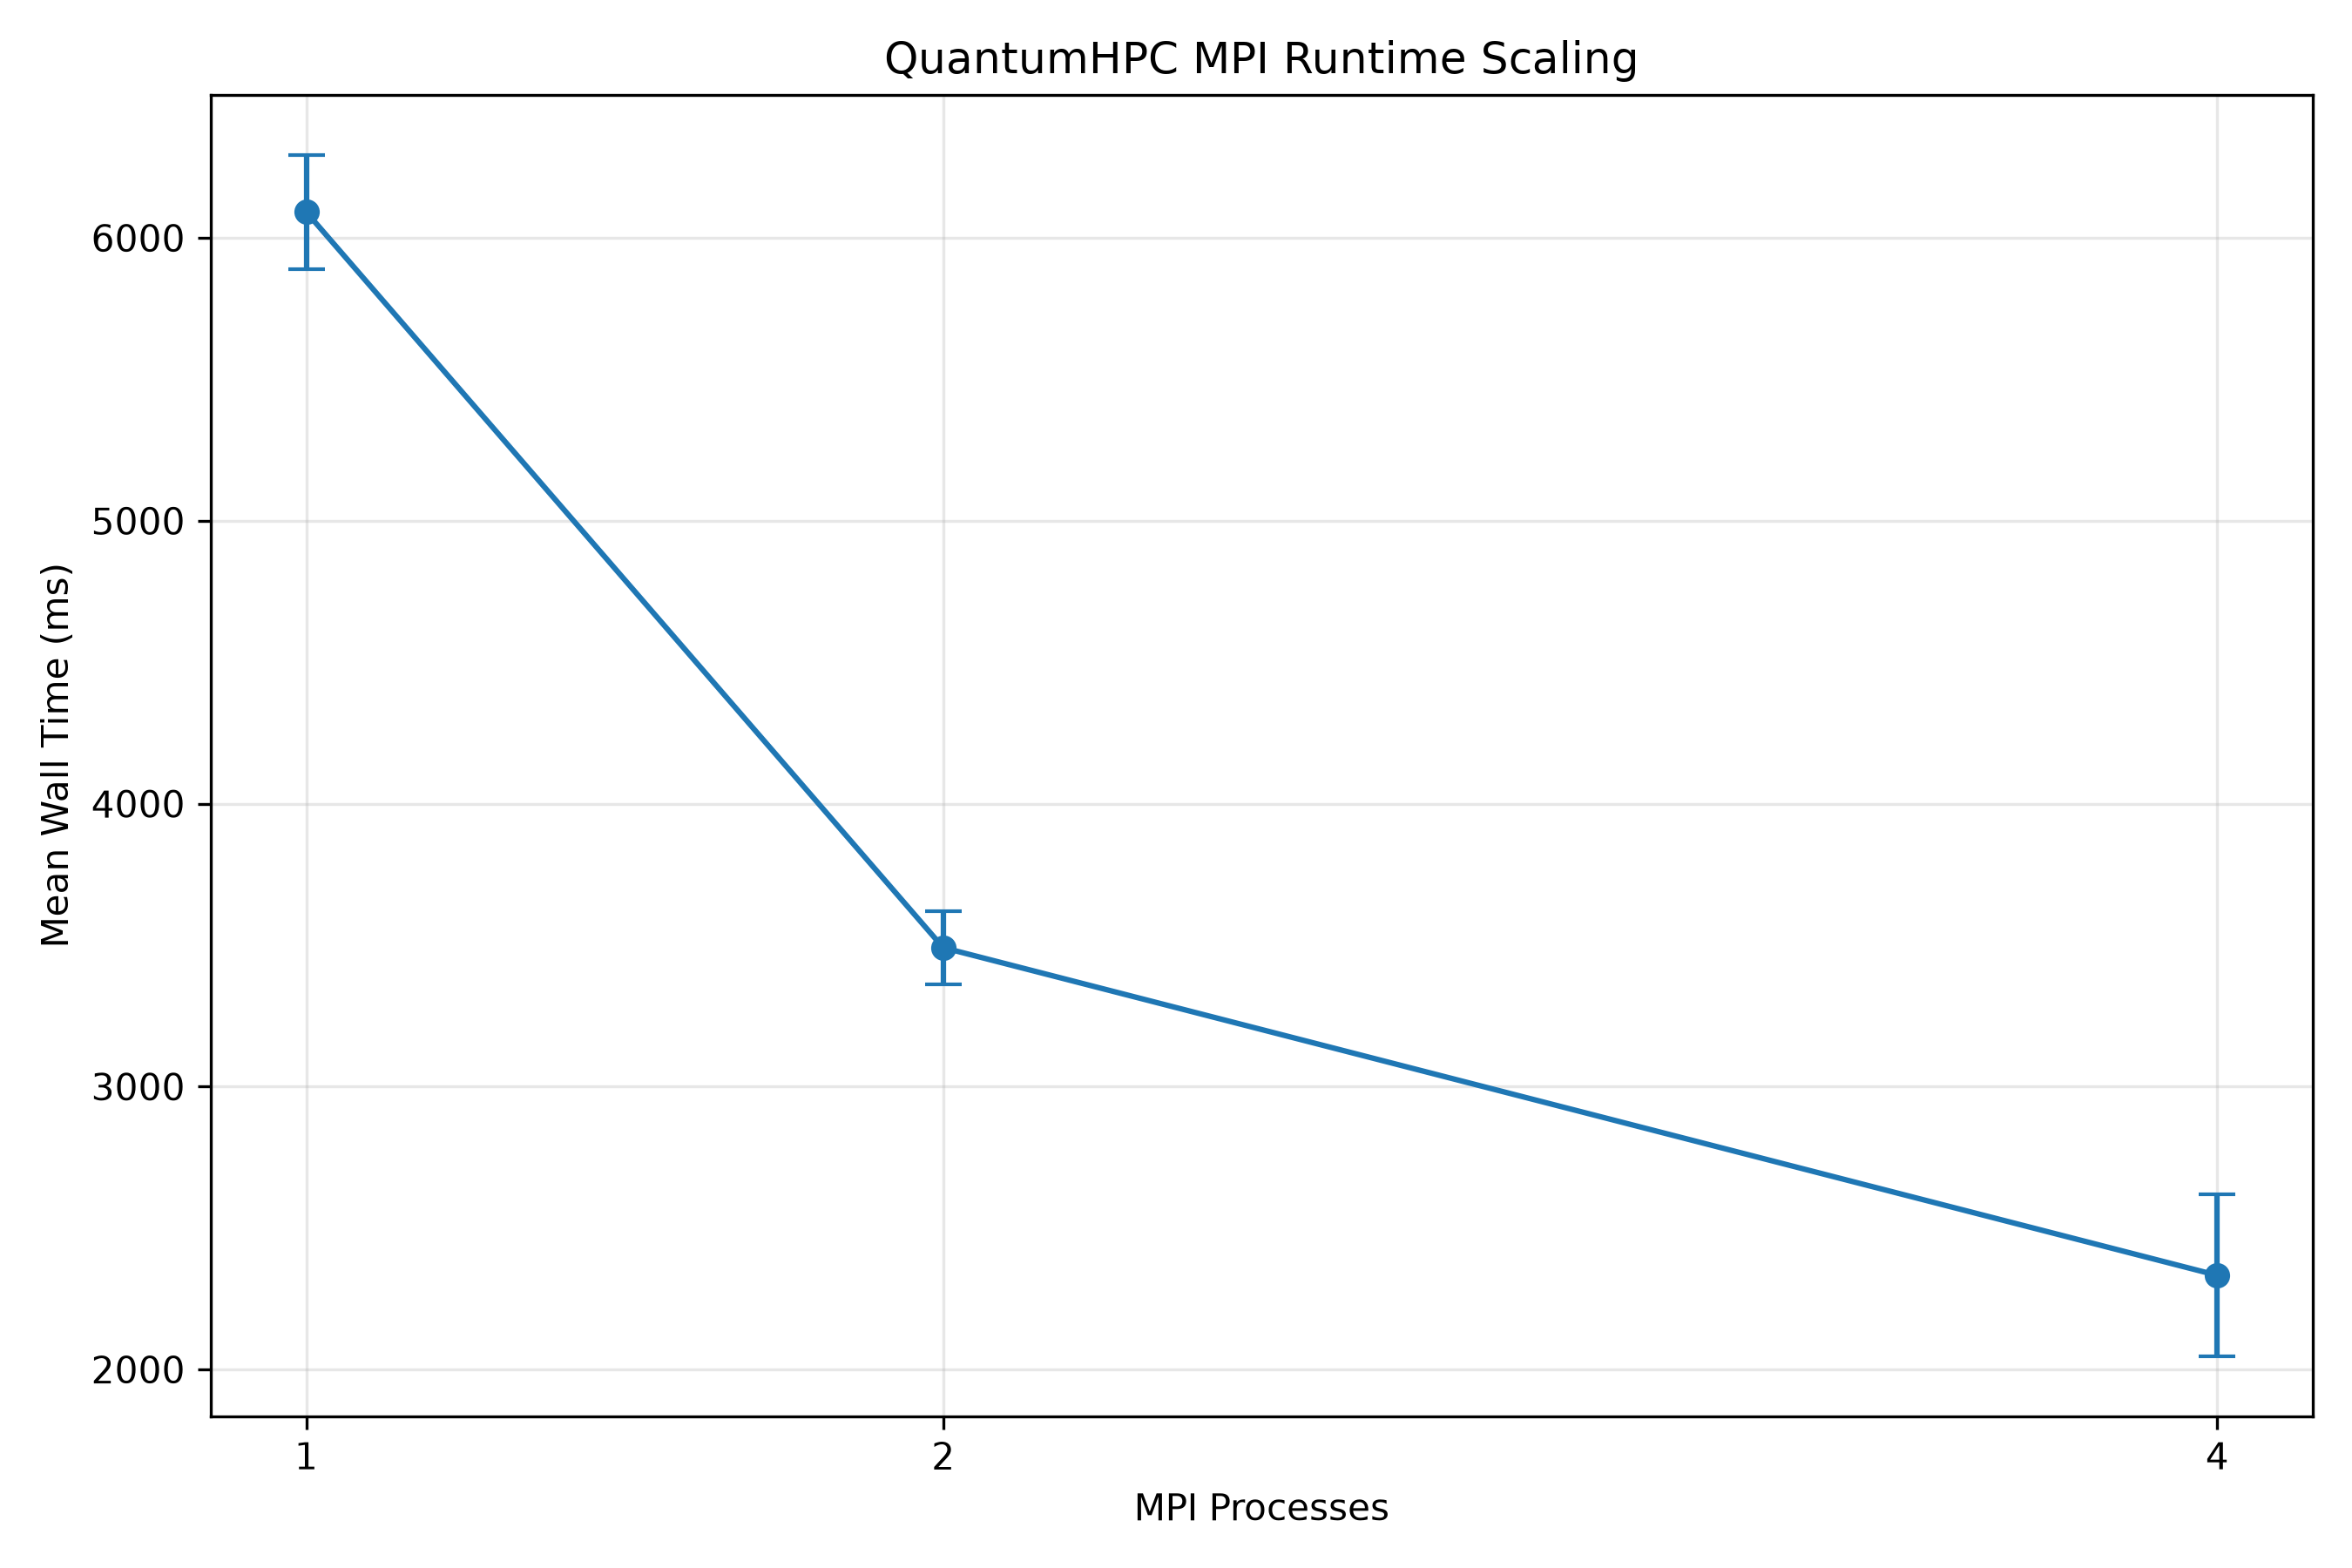
\includegraphics[width=\textwidth]{figures/mpi_runtime_scaling.png}
    \caption{Mean Bridges-2 wall time as a function of the number of MPI processes. Error bars represent the observed variation across measurements.}
    \label{fig:mpi-runtime}
\end{figure}

The corresponding measured speedup is shown in Figure~\ref{fig:mpi-speedup}. Relative to the single-process baseline, two processes produced approximately $1.74\times$ speedup, while four processes produced approximately $2.61\times$ speedup. The measured speedup therefore increased with additional MPI processes, although it remained below the ideal linear scaling of $2\times$ and $4\times$, respectively.

\begin{figure}[htbp]
    \centering
    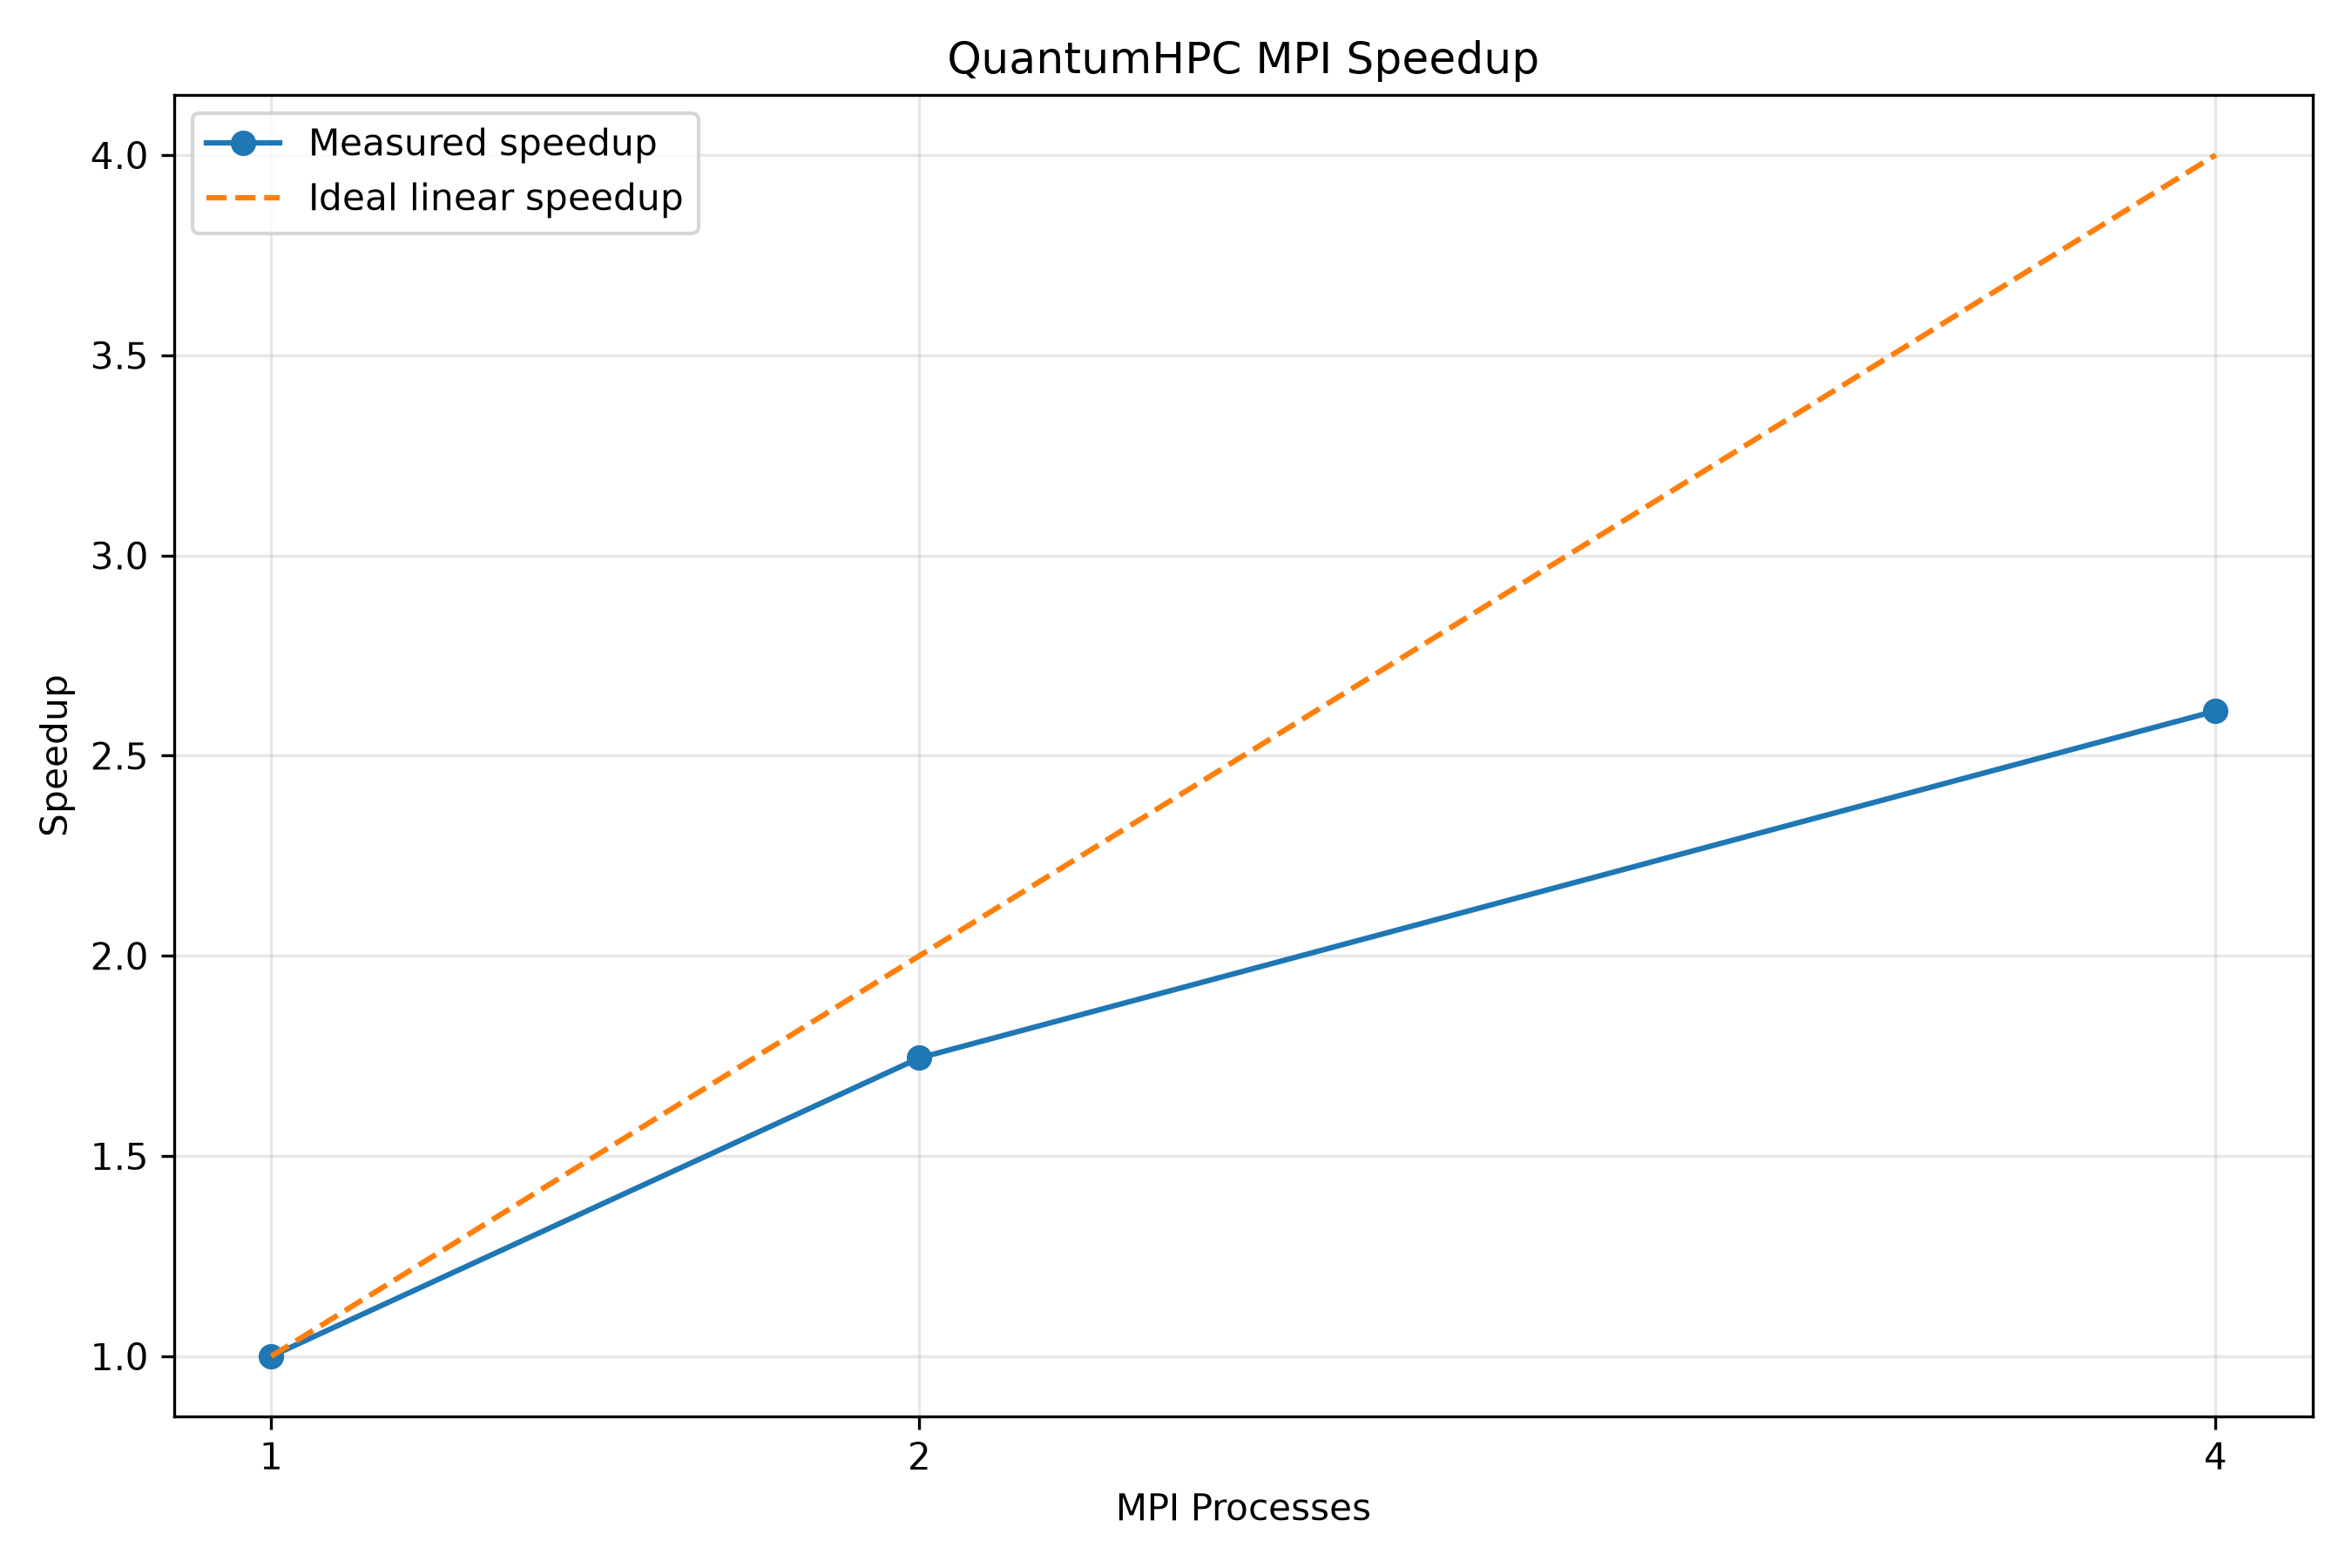
\includegraphics[width=\textwidth]{figures/mpi_speedup.png}
    \caption{Measured MPI speedup on Bridges-2 compared with ideal linear speedup.}
    \label{fig:mpi-speedup}
\end{figure}

The resulting parallel efficiency is shown in Figure~\ref{fig:mpi-efficiency}. Efficiency was approximately 100\% for one process, 87\% for two processes, and 65\% for four processes. The reduction in efficiency as additional processes are introduced indicates that the workload does not scale perfectly linearly, with communication and parallelization overhead becoming increasingly significant as the process count increases.

\begin{figure}[htbp]
    \centering
    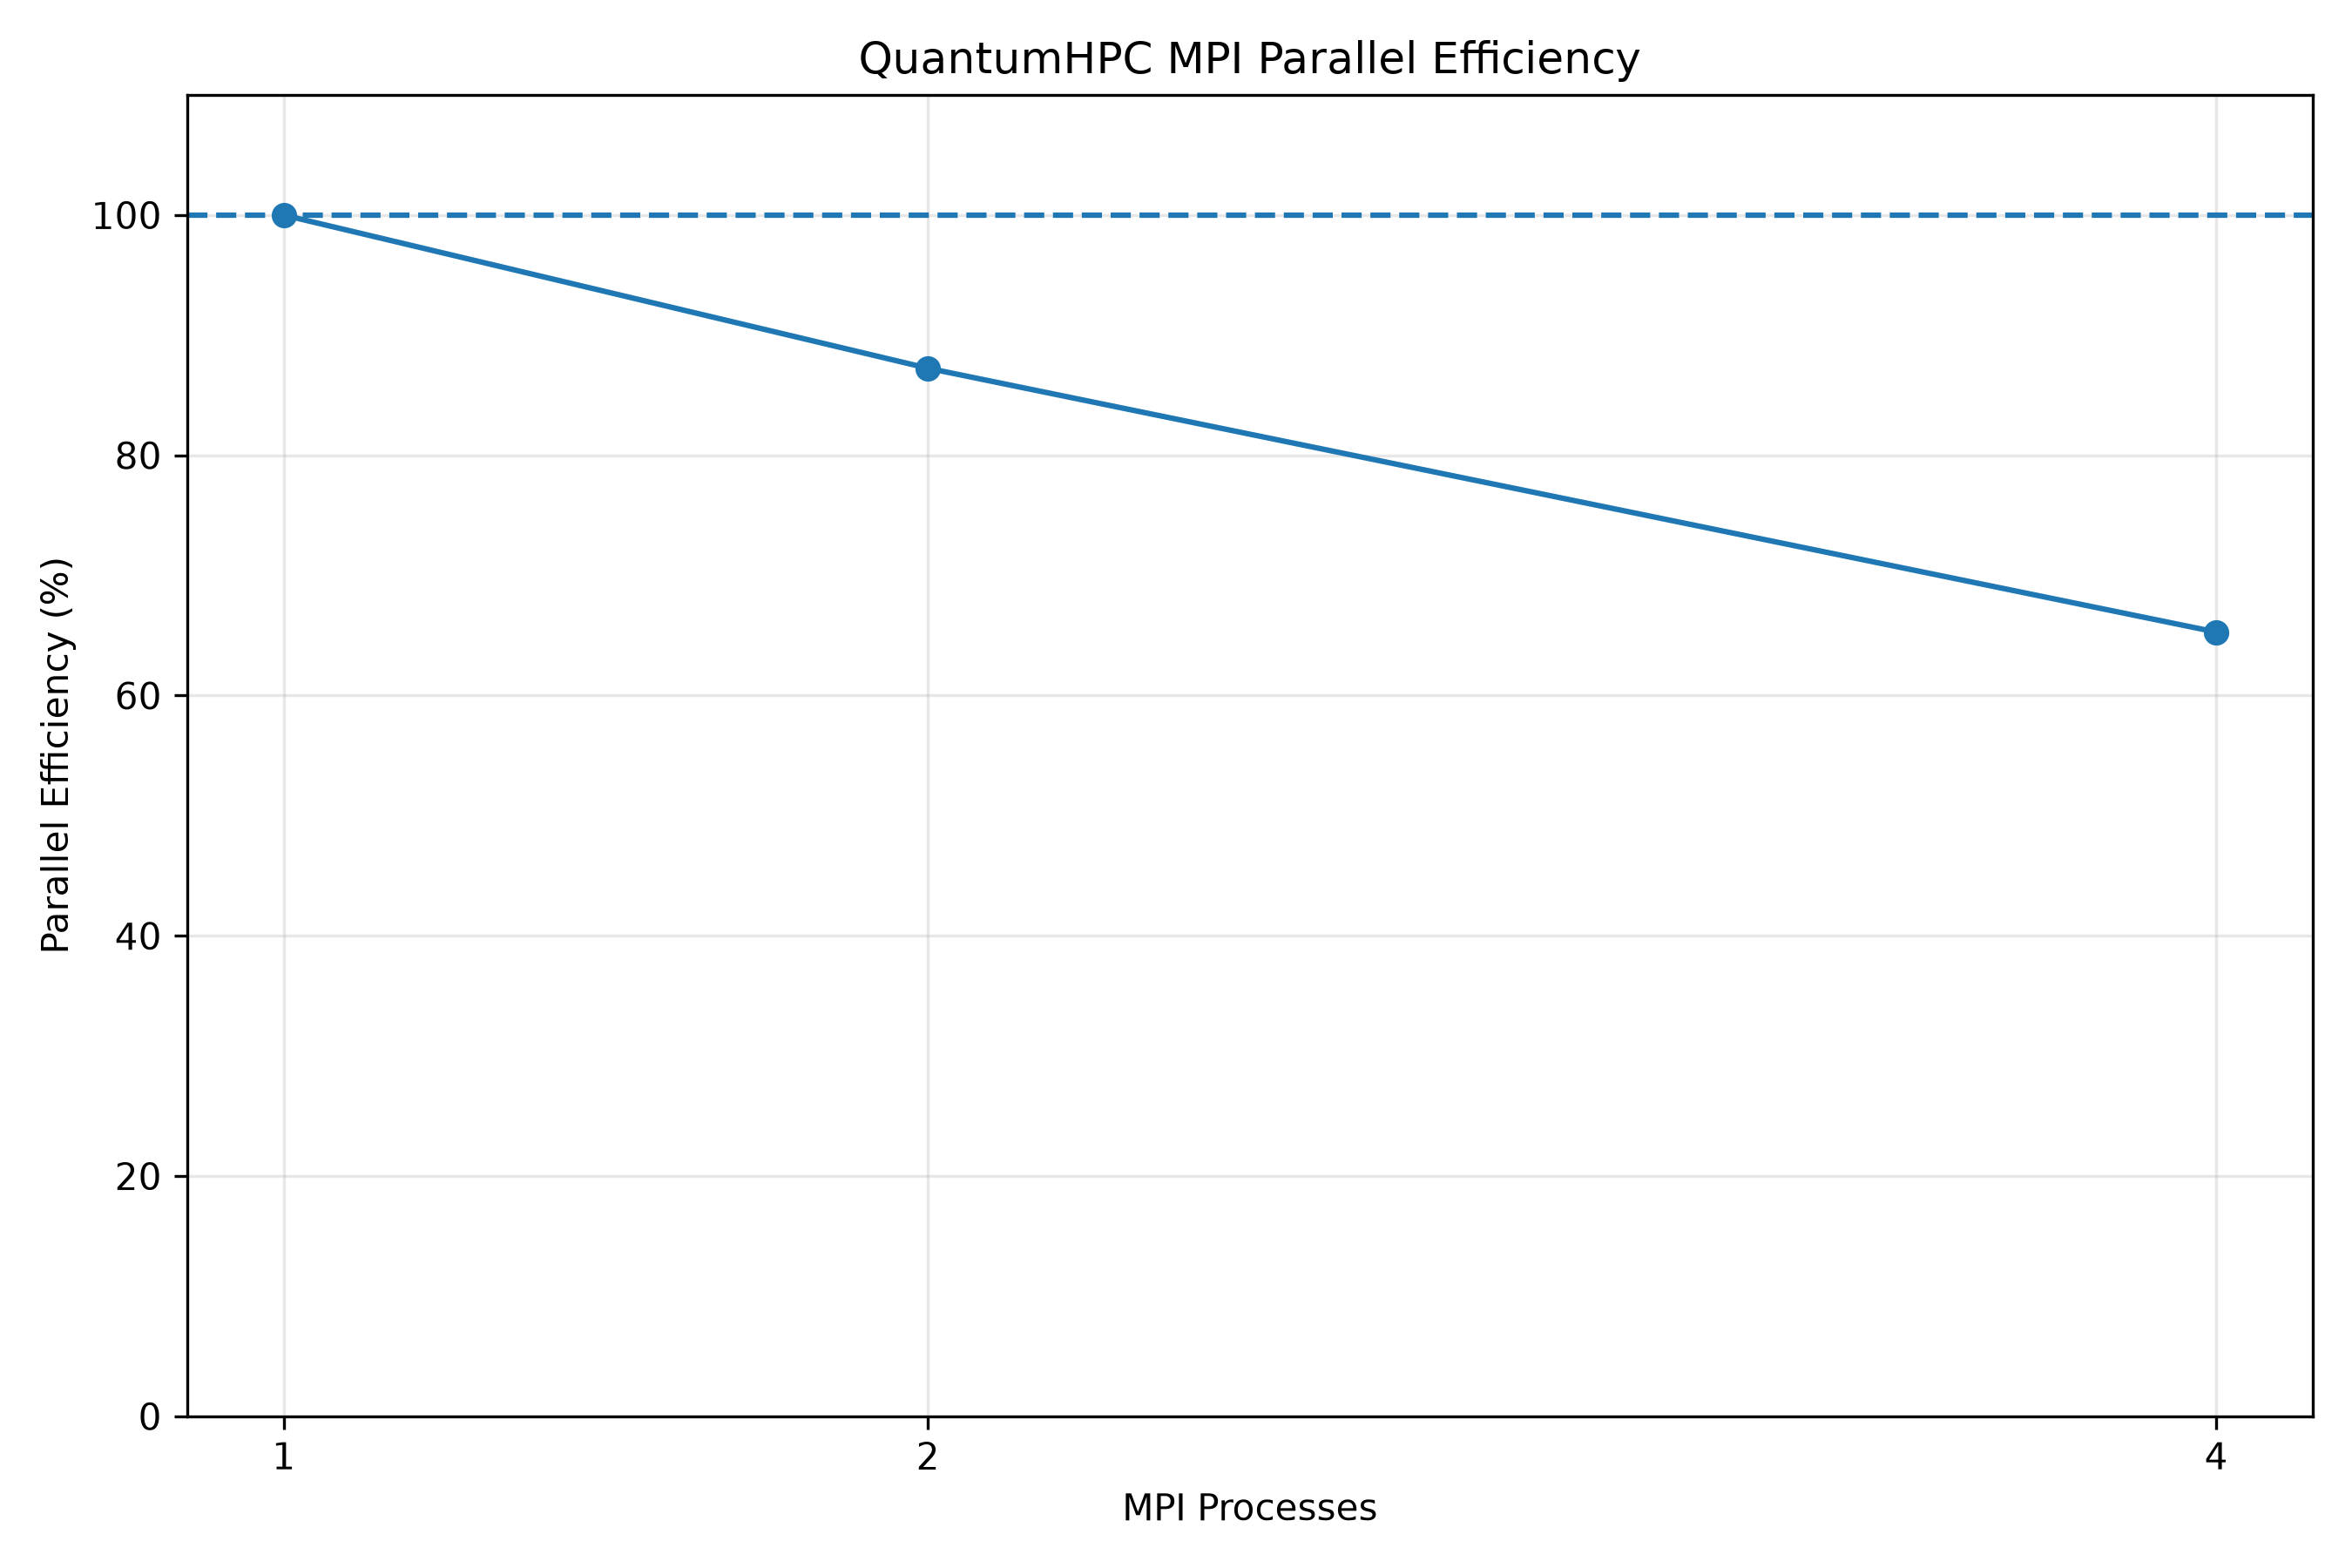
\includegraphics[width=\textwidth]{figures/mpi_efficiency.png}
    \caption{MPI parallel efficiency on Bridges-2 as the number of processes increases.}
    \label{fig:mpi-efficiency}
\end{figure}

\subsection{Discussion of HPC Scaling Results}\label{subsec:hpc-discussion}

The Bridges-2 experiments demonstrate two important aspects of the current QuantumHPC workflow. First, the parameter sweep confirms that the experimental framework can execute a controlled set of quantum-simulation conditions through the HPC environment and collect reproducible runtime measurements. The variation in simulation time across noise conditions and $\epsilon$ values provides a baseline against which later hardware and parallel-execution experiments can be compared.

Second, the MPI measurements demonstrate that distributing the workload across multiple processes reduces overall execution time. The measured speedup, however, does not remain linear as the number of processes increases. Parallel efficiency decreases from approximately 100\% with one process to approximately 65\% with four processes, indicating increasing overhead at higher process counts. These results provide an initial characterization of the scalability of the current workload and establish a baseline for subsequent larger-scale MPI experiments.

The present MPI experiment should be considered an initial scaling study rather than a final characterization of the project's distributed quantum-kernel workload. The project brief calls for larger strong- and weak-scaling experiments, including higher process counts, as the quantum-kernel computation is integrated with the broader project pipeline. Future experiments will therefore extend the current measurements to larger workloads and additional compute resources.

\subsection{Current Experimental Status}\label{subsec:current-status}

The project has progressed from initial quantum-circuit development to a functioning HPC experiment pipeline. The current workflow supports quantum-circuit construction, configurable simulation conditions, SLURM-based execution, MPI-based workload distribution, and experiment logging. The completed Bridges-2 parameter sweep established the initial CPU/HPC baseline, while the subsequent MPI experiment demonstrated measurable reductions in execution time as the number of processes increased.

The current results represent an initial performance characterization rather than the final scaling study. The 1-, 2-, and 4-process MPI experiments establish a baseline from which larger strong- and weak-scaling experiments can be developed. Additional planned work includes extending the workload to larger process counts and qubit sizes, evaluating GPU execution, comparing available HPC resources, and testing the workflow with the PhysioNet/NinaPro EMG dataset.

The remaining project work will also focus on integrating the HPC benchmarking track with the quantum-kernel and differential-privacy components developed by the other project tracks. This integration will allow the team to evaluate the complete workflow rather than treating quantum simulation, privacy, and HPC performance as independent experiments.

\section{Methodology}\label{sec:methodology}

\subsection{Quantum Simulation Framework}\label{subsec:quantum-framework}

The QuantumHPC software framework was organized as a modular pipeline for configurable quantum-circuit simulation. The main execution program accepts experiment parameters through command-line arguments and constructs an experiment configuration containing the differential-privacy parameter $\epsilon$ and the selected quantum-simulation condition. The experiment runner then uses this configuration to execute the corresponding simulation and record the experimental results.

The current experiment interface supports four values of the privacy parameter, $\epsilon \in \{1,2,4,8\}$, and three quantum-simulation conditions: noiseless, depolarizing noise, and amplitude-damping noise. These parameters provide a controlled experimental space for evaluating the simulation workflow across different configurations.

\subsection{Quantum Feature-Map Construction}\label{subsec:feature-map}

The quantum circuit component uses the ZZFeatureMap to encode classical feature data into a quantum circuit. Two implementations were developed: a library-based implementation using the Qiskit circuit framework and a manual implementation constructed from primitive quantum gates. The manual implementation provides a gate-level representation of the feature map and was developed to validate the circuit construction independently of the higher-level library implementation.

The feature-map construction is separated from the simulation backend so that the same circuit representation can be evaluated under different simulation configurations. This separation also allows the circuit-generation component to be reused as the project progresses toward larger HPC experiments.

\subsection{HPC Execution and Parameter Sweep}\label{subsec:hpc-method}

The HPC workflow was developed around the Bridges-2 computing environment and its SLURM workload-management system. MPI was selected as the distributed-memory parallelization framework for the project's scaling experiments \cite{mpiforum2023,llnlmpi}, while Bridges-2 provides the target HPC environment for the computational experiments \cite{bridges2}. The MPI environment was first validated using a four-process test program before the SLURM workflow was connected to the QuantumHPC simulation framework.

The parameter-sweep experiment evaluated four values of $\epsilon$, $\epsilon \in \{1,2,4,8\}$, under three quantum-simulation conditions: noiseless, depolarizing noise, and amplitude-damping noise. This produced twelve experimental configurations. Each configuration was submitted through the SLURM workflow, executed on Bridges-2, and recorded through the project's experiment and logging framework.

Following the parameter sweep, MPI scaling experiments were performed using 1, 2, and 4 MPI processes. Mean wall time was recorded for each process count and used to calculate measured speedup relative to the single-process baseline and parallel efficiency. The scaling measurements provide an initial assessment of the workload's behavior under distributed execution and establish a baseline for future experiments at larger process counts and on additional compute resources.

The experimental workflow separates experiment configuration, quantum-circuit construction, simulation execution, HPC job submission, and result logging. This modular organization allows the same simulation workload to be evaluated under different parameter configurations and resource allocations without modifying the underlying circuit implementation.

\subsection{Experimental Organization}\label{subsec:experimental-organization}

The experiment configuration was separated from the execution logic so that experimental parameters can be changed without modifying the simulation implementation. The main execution interface currently accepts the $\epsilon$ value and simulation condition as configurable arguments. This parameter-driven design is intended to support subsequent scaling experiments in which the workload, number of MPI processes, and compute resource can be varied systematically.

The resulting workflow separates experiment configuration, quantum-circuit construction, simulation execution, and result logging. This modular structure provides the basis for comparing serial, MPI, and GPU execution as the project progresses.

\section{Track Contributions}\label{sec:tracks}

The project is organized into three complementary tracks that address different components of the overall research problem. The Quantum Core track develops the quantum-kernel and circuit components, the Differential Privacy and Agentic MPI track addresses privacy-aware distributed processing, and the HPC Benchmarking track evaluates the computational scalability and performance of the resulting workloads. The tracks are designed to converge in the later stages of the project rather than functioning as independent experiments.

\subsection{Quantum Core}\label{subsec:quantum-core}

The Quantum Core track establishes the quantum-computing component of the project. This includes development and evaluation of the quantum feature-map and quantum-kernel methodology used to process the project's data. The track also provides the quantum workload that can subsequently be evaluated under different simulation and computing environments.

The quantum-circuit implementation developed during the initial project phase includes the ZZFeatureMap and a manually constructed gate-level equivalent. These implementations establish a controlled quantum workload that can be incorporated into the later HPC and benchmarking experiments.

\subsection{Differential Privacy and Agentic MPI}\label{subsec:dp-agentic}

The Differential Privacy and Agentic MPI track addresses the privacy and distributed-agent components of the research problem. Differential privacy is incorporated into the experimental design through the evaluation of multiple values of the privacy parameter $\epsilon$. The later Agentic MPI work is intended to connect the privacy-aware processing with distributed computational agents.

This track provides the privacy-related requirements and distributed workflow components that the HPC track must ultimately support. The current paper therefore treats the privacy experiments and the HPC execution framework as complementary components of the overall system.

\subsection{HPC Benchmarking}\label{subsec:hpc-track}

The HPC Benchmarking track addresses the computational scalability component of the research problem. Quantum-kernel and quantum-circuit simulations can become increasingly expensive as circuit size and experimental workload increase. This track therefore focuses on developing a reproducible execution and benchmarking framework capable of distributing workloads across HPC resources.

The current work has established execution on Bridges-2 through SLURM and has completed the initial 12-condition parameter sweep. MPI infrastructure has also been established as the basis for subsequent workload-distribution and scaling experiments. The planned benchmarking phase will evaluate strong and weak scaling, CPU and GPU execution, and performance across available HPC resources.

A secondary objective of this track is to evaluate the generalization of the computational workflow using the PhysioNet/NinaPro DB2 EMG dataset. This will provide an application-level test of whether the developed quantum-kernel and HPC workflow can be transferred beyond the initial clinical-data setting.

\subsection{Integration of the Tracks}\label{subsec:track-integration}

The three tracks are intended to converge into a single experimental workflow. The Quantum Core track provides the quantum workload, the Differential Privacy and Agentic MPI track provides the privacy-aware distributed-processing requirements, and the HPC Benchmarking track provides the infrastructure and performance evaluation needed to execute the workload at scale.

The integration stage will therefore evaluate not only whether the individual components function independently, but also whether they can operate together as a reproducible and scalable workflow. The resulting system will provide the basis for comparing computational performance, privacy-related behavior, and application-level generalization across the project's planned experiments.

\begin{figure}[htbp]
    \centering
    
\includegraphics[width=\textwidth]{figures/project_flowchart.png}
    \caption{Overview of the QuantumHPC project workflow, showing the progression from data processing and quantum-circuit construction through HPC execution, benchmarking, and integration of the project tracks.}
    \label{fig:project-flowchart}
\end{figure}

\section{Conclusion}\label{sec:conclusion}

This work presents the current development of a high-performance quantum simulation workflow designed to support scalable quantum machine-learning experiments. The project combines quantum-circuit construction, configurable quantum simulation, differential-privacy parameters, and HPC execution into a modular experimental framework.

The work completed to date establishes a functional computational baseline. The team developed and validated the ZZFeatureMap workflow, including a manual gate-level implementation, and established execution of the simulation framework on the Bridges-2 HPC environment through SLURM. A twelve-condition parameter sweep across four values of $\epsilon$ and three quantum-simulation conditions was completed, providing an initial CPU/HPC performance baseline.

Initial MPI experiments further demonstrated that the simulation workload benefits from distributed execution. Increasing the MPI process count from one to four reduced the measured execution time, producing measurable speedup while also revealing decreasing parallel efficiency at higher process counts. These results establish the foundation for a larger scaling study rather than representing the final performance characterization of the project.

The remaining work will extend the current experiments to larger MPI configurations and workloads, evaluate GPU execution and cross-resource performance, and investigate the application of the workflow to the PhysioNet/NinaPro EMG dataset. The three project tracks will also be integrated so that the quantum, differential-privacy, and HPC components can be evaluated as a unified workflow. These experiments will provide the additional evidence needed to evaluate the scalability and broader applicability of the proposed approach.

\backmatter

\bibliography{sn-bibliography}% common bib file
%% if required, the content of .bbl file can be included here once bbl is generated
%%\input sn-article.bbl

\end{document}
